\documentclass{article}
\usepackage{tikz}
\usetikzlibrary{arrows.meta,positioning,calc,shapes.geometric}
\pagestyle{empty}
\begin{document}
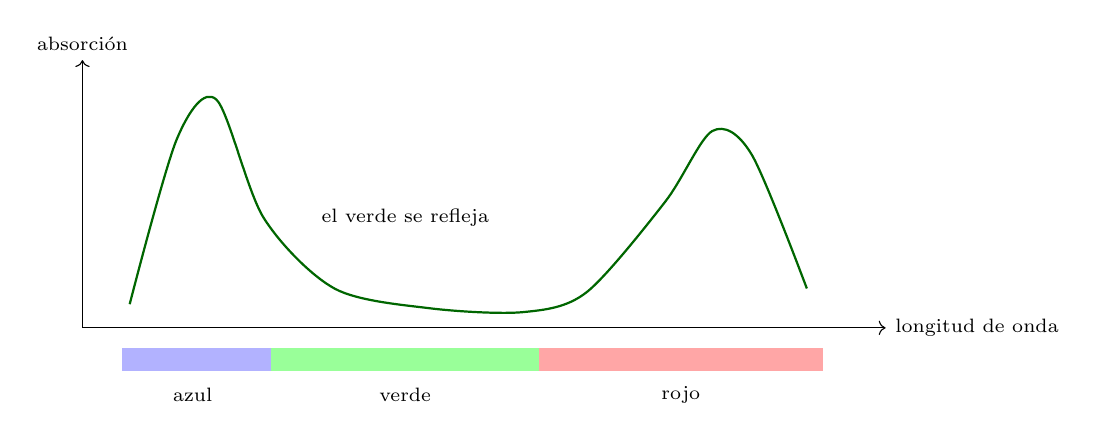
\begin{tikzpicture}

\draw[->] (0,0) -- (0,3.4) node[above, font=\scriptsize] {absorción}; \draw[->] (0,0) -- (10.2,0) node[right, font=\scriptsize] {longitud de onda};
\draw[thick, green!40!black] plot[smooth] coordinates {(0.6,0.3) (1.2,2.4) (1.7,2.9) (2.3,1.4) (3.2,0.5) (4.4,0.25) (5.6,0.2) (6.4,0.45) (7.4,1.6) (8.0,2.5) (8.5,2.2) (9.2,0.5)};
\fill[blue!30] (0.5,-0.55) rectangle (2.4,-0.25); \fill[green!40] (2.4,-0.55) rectangle (5.8,-0.25); \fill[red!35] (5.8,-0.55) rectangle (9.4,-0.25);
\node[font=\scriptsize] at (1.4,-0.85) {azul}; \node[font=\scriptsize] at (4.1,-0.85) {verde}; \node[font=\scriptsize] at (7.6,-0.85) {rojo};
\node[font=\scriptsize, align=center] at (4.1,1.4) {el verde se refleja};

\end{tikzpicture}
\end{document}
